\documentclass[landscape,12pt]{article}
\date{}
\usepackage[spanish]{babel}
\usepackage{graphicx}
\usepackage{amssymb}
\usepackage{fancyhdr}
\usepackage{multirow}
\usepackage[utf8]{inputenc}
\usepackage{fancyhdr}

\begin{document}
\renewcommand{\headrulewidth}{0.0pt}
\renewcommand{\footrulewidth}{0.3pt}
\newpage

\begin{titlepage}
	\begin{center}
		\vspace*{-1in}
		\begin{figure}[htb]
			\begin{center}
				
\includegraphics[width=8cm]{ug}
			\end{center}
		\end{figure}
		\vspace*{0.1in}
		\begin{Large}
			Ingenier\'ia en Sistemas, Inform\'atica y \\Ciencias de la Computaci\'on\\
		\end{Large}
		\vspace*{0.4in}
		\begin{LARGE}
			\textbf{\LARGE MAYALENG} \\
			\textbf{\Large Manual de Usuario} \\
			\begin{figure}[htb]
				\begin{center}
					
\includegraphics[width=4cm]{ml}
				\end{center}
			\end{figure}
		\end{LARGE}
		\begin{large}
			Autores:\\
			Douglas Figueroa \\
			Alexander Baquiax
		\end{large}
	\end{center}
\end{titlepage}
\newpage

\cleardoublepage
\listoffigures

\rfoot{
\includegraphics[width=.08\textwidth]{ml}}
\lfoot{MayaLeng}

\newpage
\pagestyle{fancy}
\begin{figure}[htb]
	\centering
	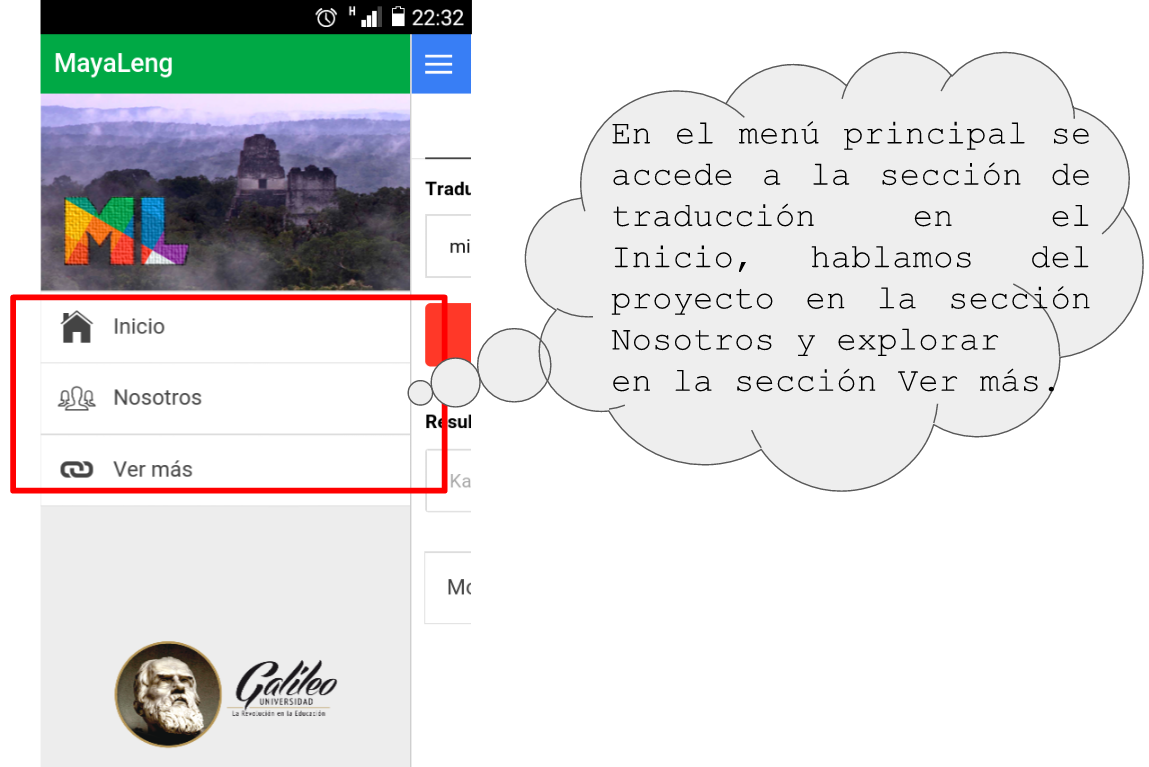
\includegraphics[width=17cm]{ml_1}	
	\caption{Menú MayaLeng}
	\label{fig:ml1}
\end{figure}
\newpage

\begin{figure}[htb]
	  \centering
	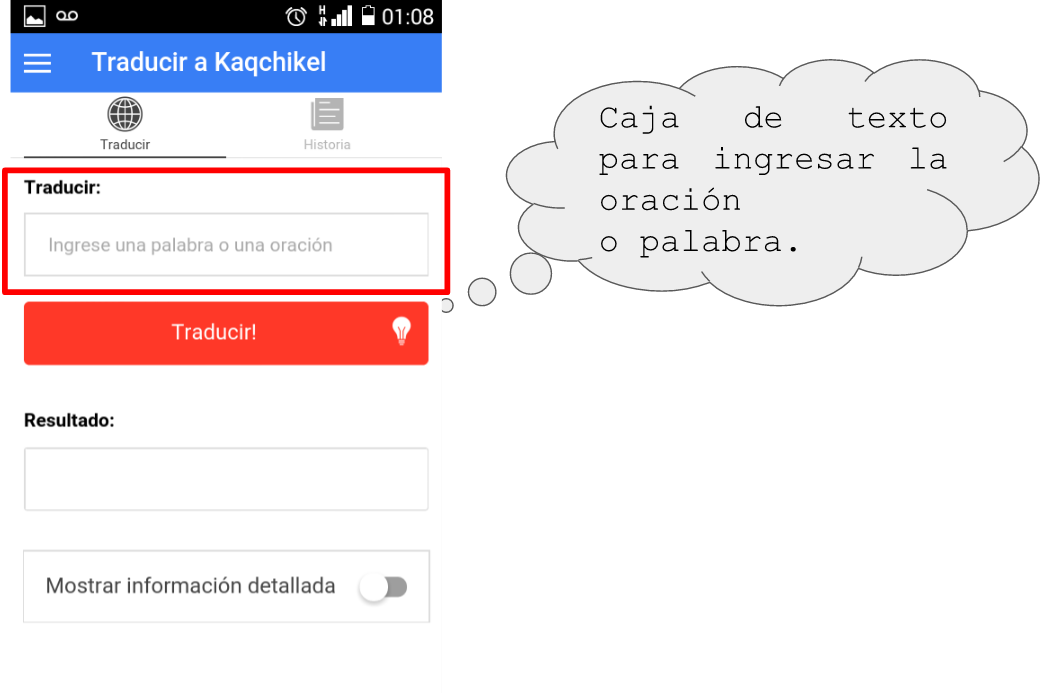
\includegraphics[width=17cm]{ml_2}
	\caption{¿Dónde ingresar el texto?}
	\label{fig:ml2}
\end{figure}
\newpage

\begin{figure}[htb]
	  \centering
	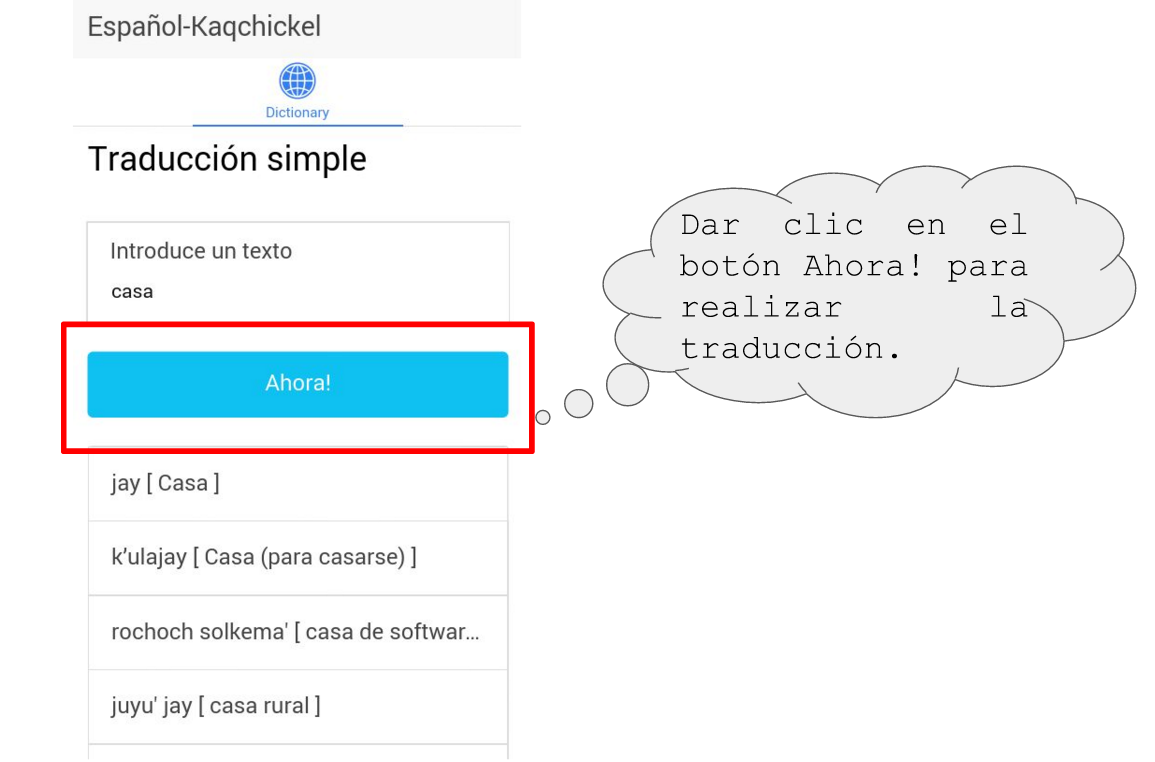
\includegraphics[width=17cm]{ml_3}
	\caption{Ingresando palabras}
	\label{fig:ml3}
\end{figure}
\newpage

\begin{figure}[htb]
	  \centering
	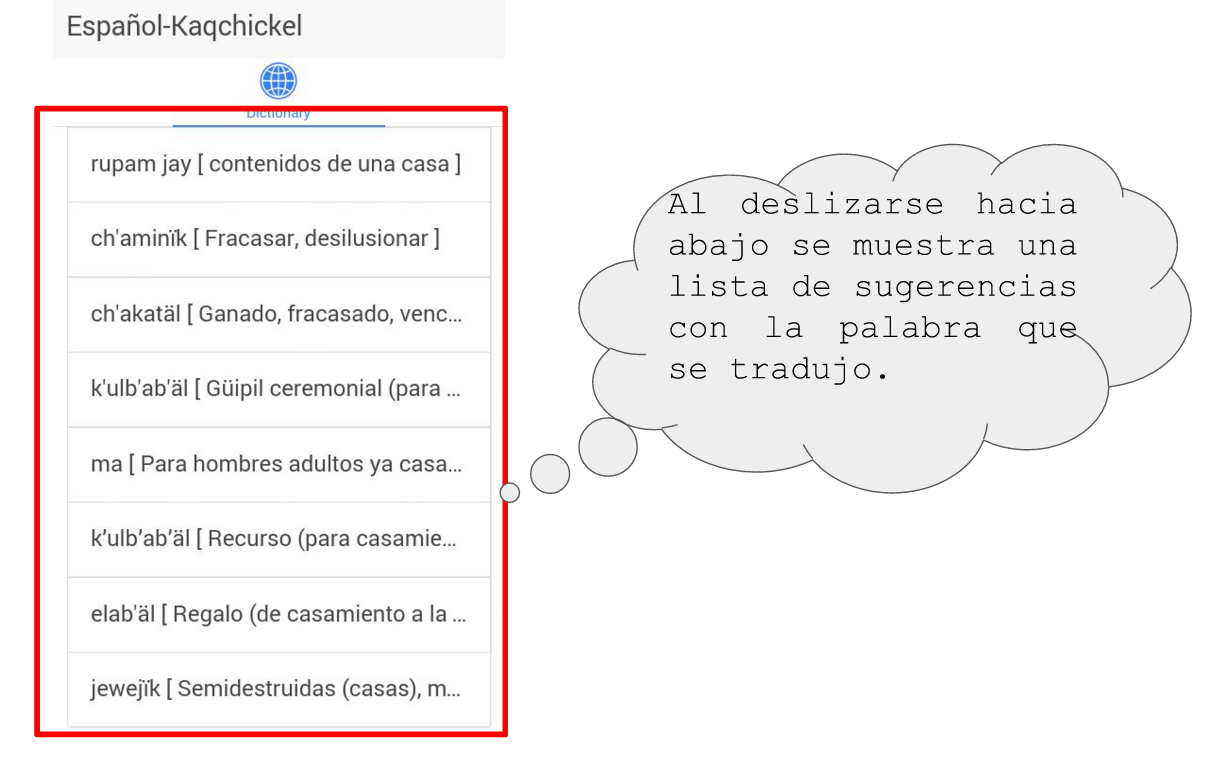
\includegraphics[width=16cm]{ml_4}
	\caption{Realizar traducción}
	\label{fig:ml4}
\end{figure}
\newpage

\begin{figure}[htb]
	\centering
	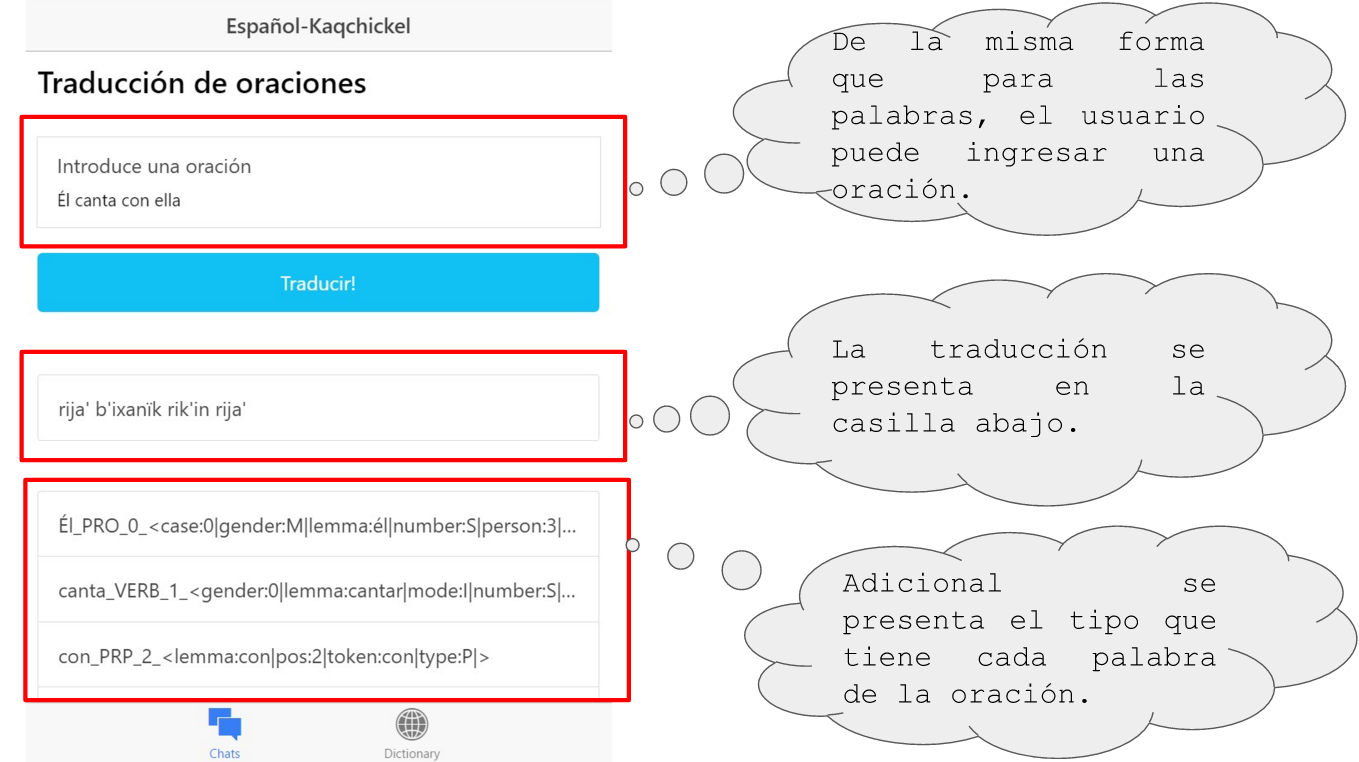
\includegraphics[width=18cm]{ml_5}
	\caption{Traduciendo oraciones}
	\label{fig:ml5}
\end{figure}
\newpage

\begin{figure}[htb]
	\centering
	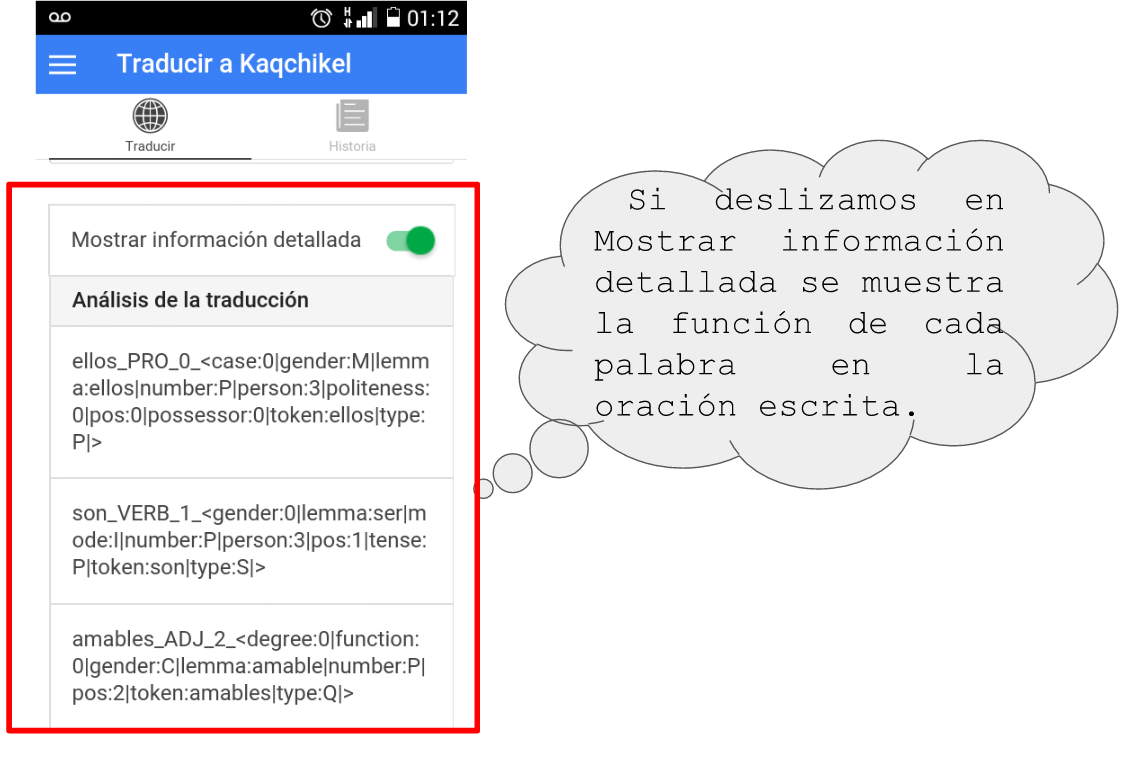
\includegraphics[width=16cm]{ml_6}
	\caption{Conociendo la estructura de la oración}
	\label{fig:ml6}
\end{figure}

\newpage

\begin{figure}[htb]
	\centering
	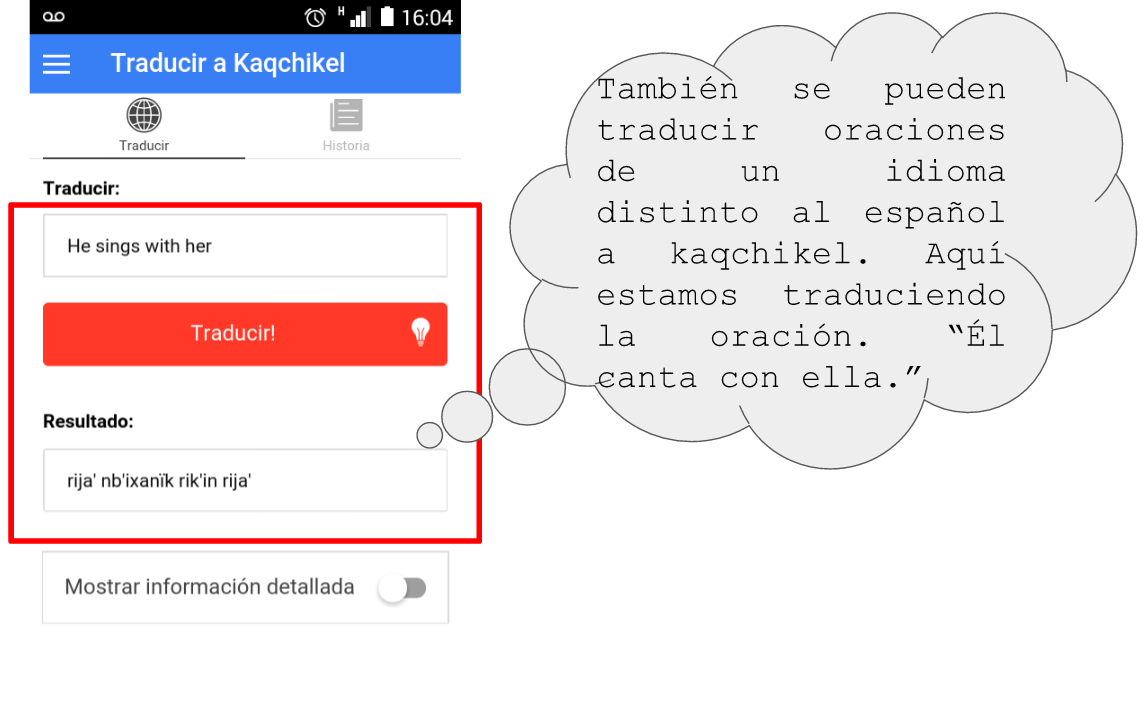
\includegraphics[width=17cm]{ml_7}
	\caption{Oraciones en otro idioma}
	\label{fig:ml7}
\end{figure}
\newpage

\begin{figure}[htb]
	\centering
	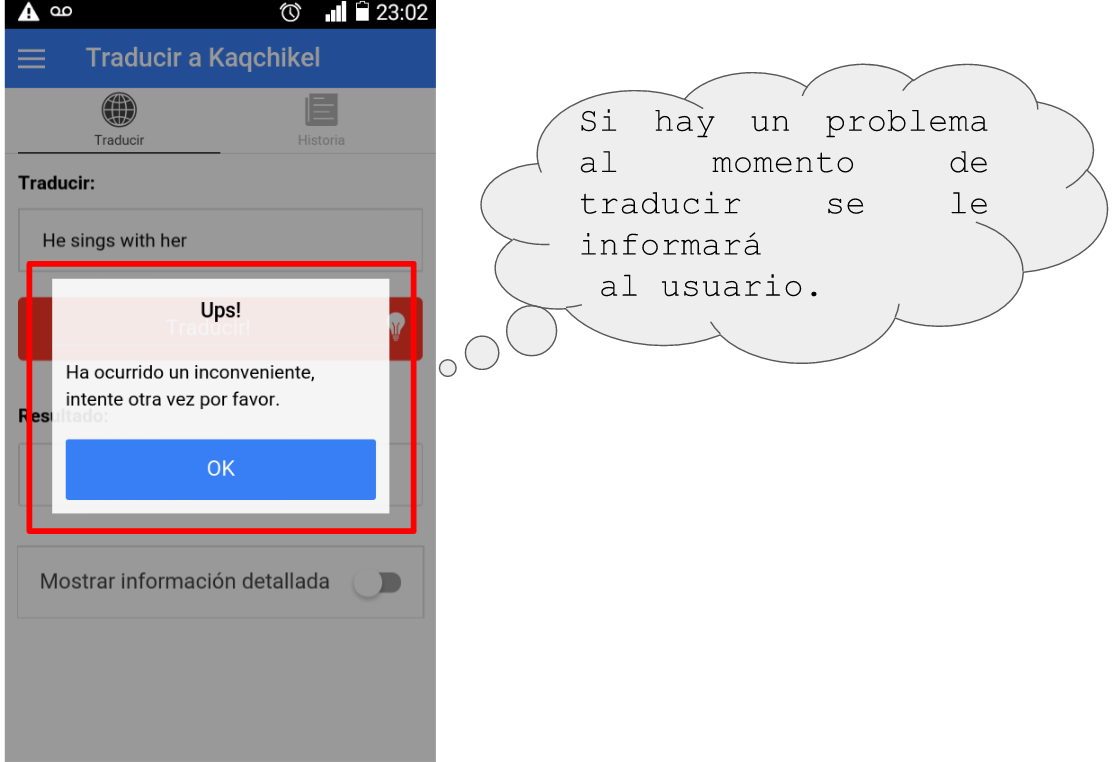
\includegraphics[width=17cm]{ml_8}
	\caption{Alertas}
	\label{fig:ml8}
\end{figure}
\newpage
\end{document}